\documentclass[aps,prc,twocolumn,showpacs,floatfix,nofootinbib,preprintnumbers,superscriptaddress,amsmath,amssymb]{revtex4-1}

\usepackage{wrapfig}

\bibliographystyle{apsrev}

\ifx\pdfoutput\undefined
\usepackage[dvips]{graphicx}
\else
\usepackage[pdftex]{graphicx}
\pdfcompresslevel=9
\fi
\usepackage{epstopdf}


\newcommand{\OP}[1]{{\bf\widehat{#1}}}

\newcommand{\be}{\begin{equation}}

\newcommand{\ee}{\end{equation}}

\begin{document}

\pagestyle{plain}

\section*{Master Thesis project for Giovanni pederiva: determination of the topological charge and susceptibility 
from lattice QCD and the gradient flow}

The Standard Model of Particle Physics (SM) has been widely successful in describing 
the measured particle spectrum and composition of matter ranging from quarks and gluons 
to multi-hadron systems.  Such systems constitute approximately 5\% of the observable 
matter-energy within the Universe.  Yet the theory alone cannot explain the origins of 
the remaining 95\% of matter and energy, dubbed `Dark Matter' and `Dark Energy', respectively.  
Further, the SM does not provide the requisite amount of charge conjugation and parity (CP) 
symmetry violation to account for the observed matter/anti-matter asymmetry.  Therefore any physical description of such 
phenomena requires a theory that goes \emph{beyond} the Standard Model (BSM), while at the 
same time encompassing the Standard Model and its predictions related to ordinary matter.

There are numerous candidate BSM theories and a description of these theories is 
beyond the scope of this project.  However, these theories all share certain operator 
traits that can be utilized in a formal study involving numerical methods of 
quantum chromodynamics (QCD), the gauge theory describing the strong interactions.  
When viewed as a low-energy effective theory of some larger (still unknown) fundamental theory, 
the SM, consisting of renormalizable operators of dimension 4 or less, 
is augmented with BSM operators of dimension $>$ 4.  The structures of these higher 
dimensional operators can be determined generically assuming the larger fundamental theory 
respects certain symmetries (e.g. the combined charge conjugation, parity and time reversal (CPT) invariance). 
Different candidate BSM theories will give different couplings for these higher-dimension operators.  When BSM theories 
are expressed in this manner, all the benefits inherent to effective field theories (EFTs) follow through, 
such as a hierarchy in operator complexity and a systematic power counting of terms.

Because of the generality of these higher-dimension operators, 
calculations of these operators can be performed with their unknown coefficients as free parameters using lattice QCD (LQCD), 
to be later fixed by candidate BSM theories.  
Conversely, a phase-space investigation of these parameters can be studied to rule-out different BSM theories.  
The study of these higher-dimension operators with a lattice regulator is plagued by 
hard renormalization ambiguities. 
The lattice discretized version of these higher-dimension operators can cause mixing of their coefficients 
with lower-dimension operators, making the separation and extraction of BSM observables from standard QCD observables very difficult.  
To address this issue, we have proposed a new method~\cite{Shindler:2014oha,Shindler:2015aqa} 
based on the use of the gradient flow~\cite{Luscher:2010iy,Luscher:2013cpa} 
to circumvent such mixing, as well as to address other issues related to renormalization.

The overall goal of this research program is to calculate nuclear observables induced by these general BSM operators using lattice QCD.  
Such observables include the electric dipole moment (EDM) of nucleon and few-body nuclear systems. 
In this thesis project we focus on the part of the calculations related to the
CP violation within the Standard Model. 


\section*{CP violation within the Standard Model and electric dipole moments}
The EDMs of the neutron and proton are very sensitive probes of CP-violating sources 
beyond those contained in the SM.
In fact, the current bound on the neutron EDM strongly constrains many models of BSM physics. 
At current experimental accuracies, a nonzero nucleon EDM cannot be accounted for by the phase 
in the quark-mass matrix. 
This implies that such a signal is either caused by a nonzero QCD $\theta$ term or 
by genuine BSM physics which, at low energies, 
can be parametrized in terms of higher-dimensional CP-violating quark-gluon operators. 
Irrespective of the origin, the signal for the nucleon EDM will be small and largely 
masked by strong-interaction physics, which presents a formidable challenge to the interpretation
of such a signal.
To disentangle the origin of a nonzero EDM measurement (e.g. $\theta$ term or BSM), 
a quantitative understanding of the underlying hadronic physics is required.

In the presence of $N_f$ fermions, the general QCD Lagrangian in Euclidean space with a $\theta$ term
reads
\begin{equation}
{\cal L_\theta}= {1\over 4} F_{\mu\nu}^a(x)F_{\mu\nu}^a(x)
+ \bar\psi\, D \psi
+ \bar\psi_L \,M\,\psi_R + \bar\psi_R \,M^\dagger\,\psi_L
- i \theta_q q(x),
\end{equation}
%\begin{equation}\label{QCD1}
%\mathcal L_{\mathrm{QCD}} = -\frac{1}{4}G_{\mu\nu}^aG^{a,\mu\nu} + \bar\Psi(i\Dslash{D} - M)\Psi - \theta_q \frac{g^2}{64\pi^2}\epsilon^{\mu\nu\alpha\beta} G^a_{\mu \nu}G^a_{\alpha \beta}\,\,\,,
%\end{equation}
where $\psi$ is an $N_f$ component vector in flavor space, $M$ is the
quark mass matrix, and $q(x)$ is the topological charge density.  The parameter
$\theta_q$ and the imaginary part of the quark mass are related, so that the
relevant $\theta$ parameter is given by
\begin{equation}
\theta = \theta_q + {\rm arg}\,{\rm det}\, M.
\label{thetafe}
\end{equation} 
This term is CP-violating and induces, for example,  an electric dipole moment within the neutron.    
One of the most stringent constraints on possible violations of parity and time reversal 
(equivalently CP symmetry assuming CPT invariance) symmetries is inferred from
measurements of the neutron EDM.  

The current experimental limit on the neutron EDM is $|d_N|<2.9 \cdot 10^{-13}~e \,{\rm fm}$~\cite{Baker:2006ts} 
and experiments are underway to improve this bound by one to two orders of magnitude.
In fig.~\ref{fig:dn_history} we show the history of neutron EDM limits from experimental measurements.
The bound on the proton EDM is induced from the $^{199}{\rm Hg}$ EDM limit~\cite{Griffith:2009zz} 
and is $|d_P|<7.9 \cdot 10^{-12}~e\,{\rm fm}$. Recently the bound on the $^{225} {\rm Ra}$ EDM has also improved 
dramatically~\cite{Bishof:2016uqx}, $\left|d(^{225} {\rm Ra})\right| < 1.4 \cdot 10^{-10} e$ fm.
While this specific measurement is not competitive at the moment with the $^{199}{\rm Hg}$ one
it has the potential to achieve rapid improvements by many orders of magnitude through a series of experimental upgrades. 
Plans exist to probe the EDM of the proton directly (and other light nuclei) in storage rings \cite{Pretz:2013us} with a 
proposed sensitivity of $10^{-16}~e \cdot {\rm fm}$, thus improving the current bounds 
by several orders of magnitudes and covering a wide range where BSM physics can show its footprint.
Test of fundamental symmetries and the measurement of atomic EDMs represent one of the main research thrusts 
of FRIB. Specific rare isotopes produced at FRIB, such as $^{229} {\rm Pa}$ and $^{225}{\rm Ra}$ 
are expected to have a much larger EDM than most atoms providing an ideal environment to improve
dramatically the current upper limits.
There is a huge effort underway to improve limits or find EDMs like the experimental proposals
(p,d)EDM experiment at BNL, the neutron EDM experiment at ORNL, ILL, FRM-2,
FNAL,PSI/KEK/TRIUMF, the charged particle (d, p)EDM at COSY
and the lepton EDM at J-PARC, FNAL aiming at a sensitivity of $10^{-16}\,e$ fm.
\begin{figure}
%  \begin{center}
    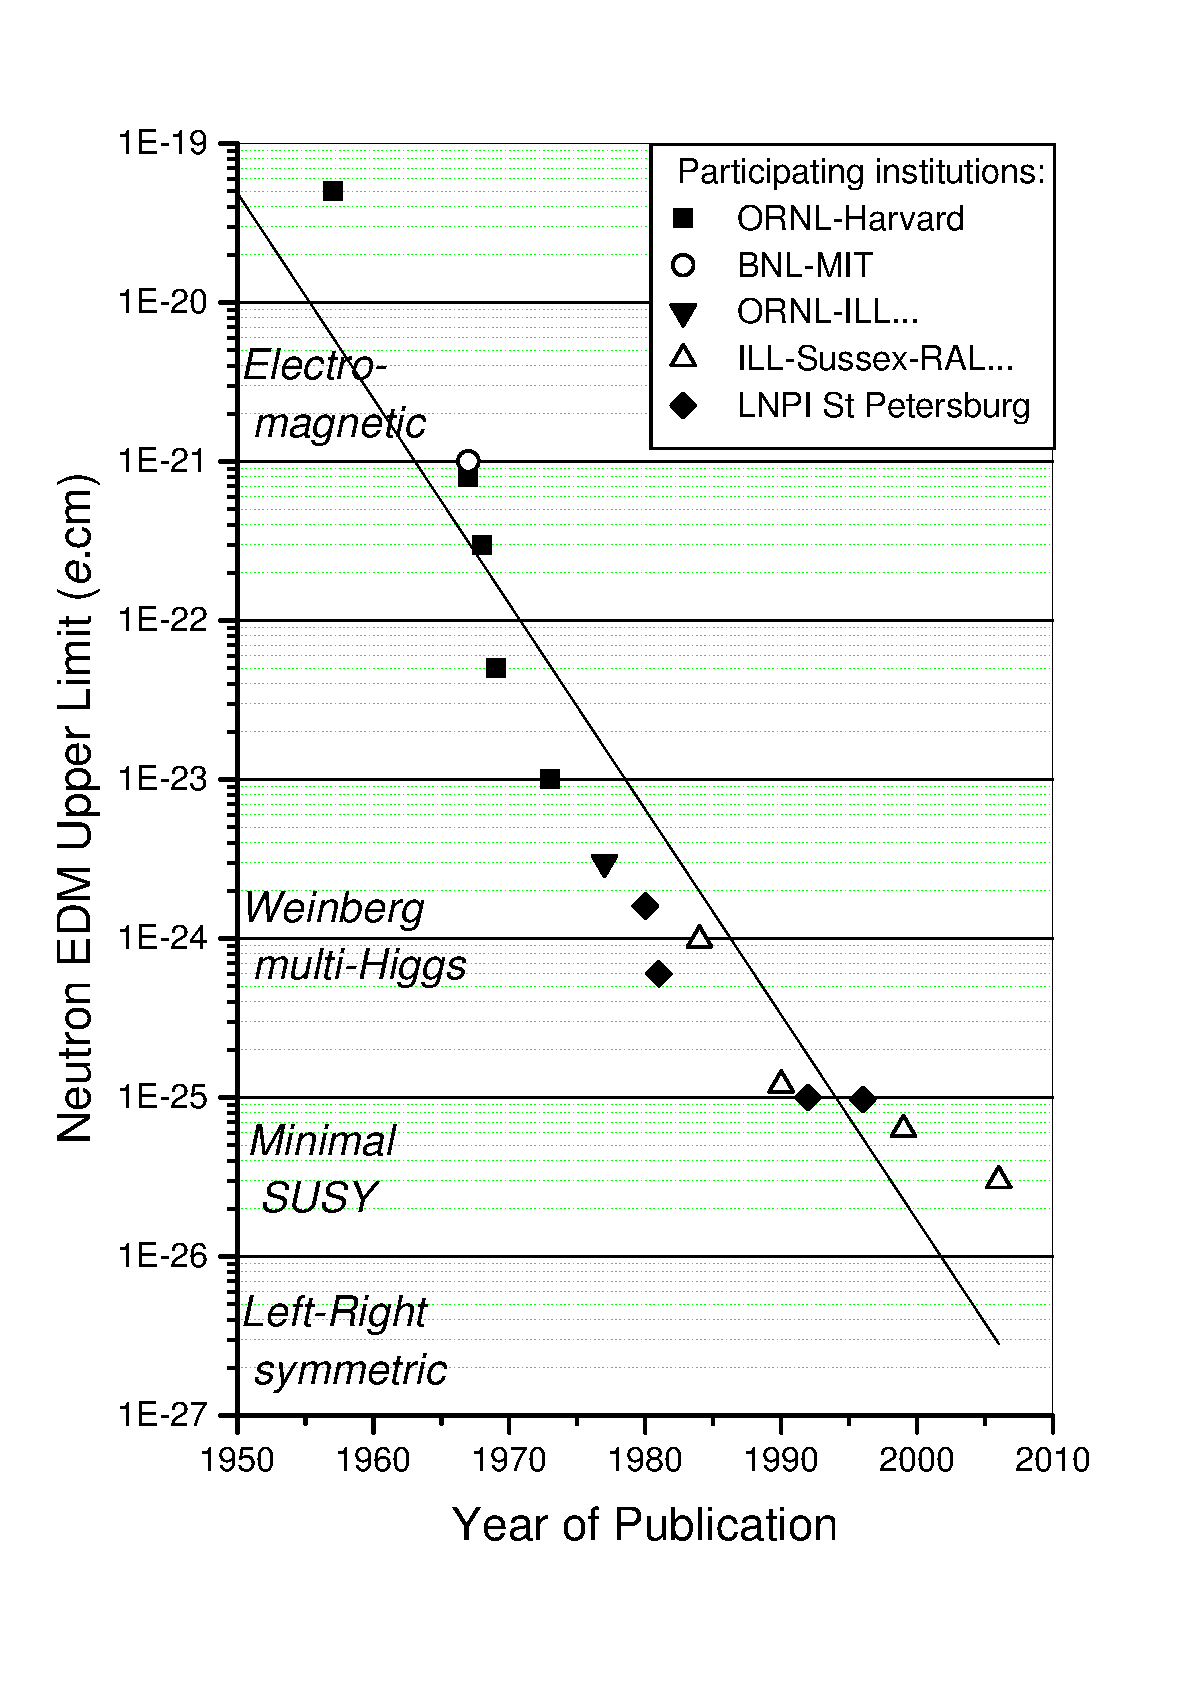
\includegraphics[width=.45\textwidth]{fig01_edm_limit.pdf}
%  \end{center}
\vspace{-1.5cm}
  \caption{History of neutron EDM limits. Figure from ref.~\cite{Harris:2007fz}.}
  \label{fig:dn_history}
\end{figure}
In order to translate the above experimental bound into a constraint on
$\theta$ and CP-violating BSM operators, one needs to compute their contribution to 
the nucleon or deuteron EDMs.
Nucleon EDMs arising from the QCD $\theta$ term or BSM physics have been calculated both in 
models~\cite{Pospelov:2005pr} and in chiral perturbation theory~\cite{Ottnad:2009jw,Mereghetti:2010kp}. 
In the latter approach, the nucleon EDMs are calculated 
in terms of effective CP-odd hadronic interactions that have the same symmetry properties 
as the underlying CP-odd sources at the quark level (for a review, see \cite{Mereghetti:2015rra}). 
The calculated EDMs depend on several low-energy constants (LECs) whose sizes are in most 
cases unknown and need to be estimated or calculated with lattice QCD.
 
Lattice QCD can thus be used to perform an {\it ab initio} calculation of the nucleon 
and light nuclei EDMs.
For the $\theta$ term, this has already been shown in the pioneering works 
in refs.~\cite{Shintani:2005xg,Berruto:2005hg} and later in ref.~\cite{Shintani:2008nt,Aoki:2008gv} 
(for BSM sources only the nucleon EDMs arising from the quark EDMs have been calculated 
with lattice QCD \cite{Bhattacharya:2015esa}).
%The chiral and infinite volume extrapolations of unpublished lattice data from Shintani et al. 
%have been performed in refs.~\cite{Guo:2012vf,Akan:2014yha}.
The calculation of the EDM within a lattice (discretized) formulation of QCD 
is very non-trivial, and presents, together with the standard LQCD systematics, large difficulties for two main reasons. 
The renormalization of the CP-odd operators and the degradation of the signal-to-noise ratio towards the chiral limit.
Additionally, the $\theta$ term itself introduces an imaginary term in the real Euclidean action,
which produces a sign problem and precludes the use of standard stochastic methods employed by lattice QCD.  

\section*{The Gradient flow}

In this section we give a short introduction to the gradient flow that is at the base of the
method we propose to use for this project.
The gradient flow (GF), for gauge~\cite{Luscher:2010iy} 
and fermion~\cite{Luscher:2013cpa} fields, used in combination with a lattice regulator, 
can probe the non-perturbative dynamics of QCD
in advantageous manners.
It is defined by a differential equation that gauge and fermion
fields satisfy as a function of the space-time coordinates $x$ and of a new
scale, the flow time $t$.

The works by L\"uscher and Weisz~\cite{Luscher:2010iy,Luscher:2011bx,Luscher:2013cpa}
give us a complete understanding of the continuum limit
of observables at non-vanishing flow time. This allows us to use the GF
to define observables that otherwise would be difficult
to compute with standard methods.
For example the GF has been used to give operational definitions to the
fundamental parameters of QCD as the strong coupling~\cite{Luscher:2010iy,Fodor:2012td,Fritzsch:2013je}
or other quantities, as the chiral condensate~\cite{Luscher:2013cpa}
and the energy-momentum tensor~\cite{Suzuki:2013gza,DelDebbio:2013zaa}.
The GF can also be used to define new relative ways to set the scale in 
lattice QCD calculations~\cite{Luscher:2010iy,Borsanyi:2012zs}.

In particular the topological susceptibility~\cite{Luscher:2010iy} and the chiral condensate~\cite{Luscher:2013cpa}
can be computed with rather high precision because with the gradient flow 
mixing with lower-dimensional operators can be avoided.
Local operators at non-vanishing flow time have a very simple renormalization pattern~\cite{Luscher:2010iy,Luscher:2011bx,Luscher:2013cpa},
but to relate them with the operators at vanishing flow time one has to rely to 
Ward identities (WI)~\cite{Luscher:2013cpa,DelDebbio:2013zaa,Shindler:2013bia} or to the small flow-time expansion.

The goal of this project is to use the gradient flow to define and compute all the 
possible CP-violating contributions to the EDM of nucleons and few-body nuclei.
This is possible because the gradient flow allows 
a direct calculation of the topological charge density at non-vanishing flow time
and, in combination with a small flow-time expansion, the simplification
of the renormalization pattern of higher-dimensional operators. 

The results will be published in scientific journals, if possible.

\section*{Progress plan and milestones}
The aims and progress plan of this thesis are as follows
\begin{itemize}
\item Fall 2017: study the gradient flow for gauge fields~\cite{Luscher:2010iy} and fermions~\cite{Luscher:2013cpa}.
\item Fall 2017: implement the code that reads in the gauge configurations.
and then computes the gradient flow for gauge fields.
\item Spring 2018: compute the flow-time dependence of the topological charge and the topological susceptibility. 
\item Spring 2018: combine the calculation of the topological charge with existing calcualtion of fermionic contractions
to extract the $\theta$-term contribution to the nucleon EDM.
\item Spring 2018: The last part deals with a proper write-up of the thesis. 
\end{itemize}
 

The thesis is expected to be handed in May/June 2018.


%\bibliographystyle{apsrev}
\bibliography{references}



\end{document}












